\chapter{Aufbau und Systemarchitektur}

\section{Systemarchitektur – Web-Applikation}

\section*{Erklärung}
Die Systemarchitektur der Webanwendung besteht grundsätzlich aus zwei Teilen. Dem auf NGINX [\ref{sec:NGINX}] basierenden Server und dem Client der per Browser die Seite aufruft. Beim Bad-Designer handelt es sich um eine HTML-Seite mit JavaScript und nicht um eine auf einem Framework basierende Applikation.
Auf dem Server sind alle benötigten Dateien und die Logik. In den Dateien, die in JavaScript geschrieben wurden, befinden sich die Modelle, die Animationen und die Geschäftslogik. Diese werden dann an den Browser übermittelt und gerendert.

\section*{Deployment}
Um die Aufwendung auf einem Server zu deployen und um sie anschließend zu verwenden, müssen einige Kriterien erfüllt werden. Es muss ein NGINX-Server [\ref{sec:NGINX}] vorliegen auf dem die index.html und die JavaScript Dateien hochgeladen wurden. Erst diese ermöglichen den Start der Anwendung, zusätzliche Schritte sind nicht von Nöten.

\begin{figure}[b]
    \centering
    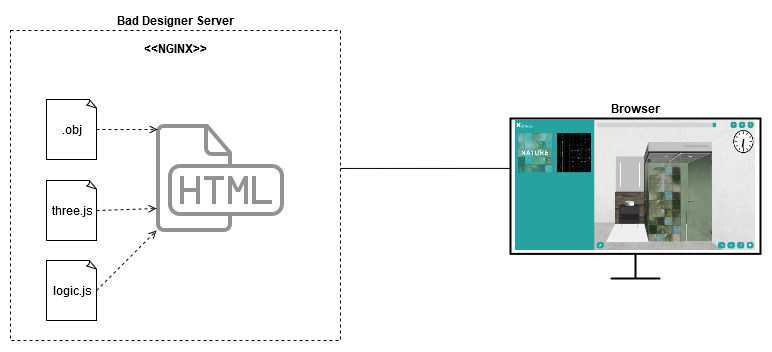
\includegraphics[width=0.6\textwidth]{images/DA-SysArch.jpg}
    \caption{Systemarchitektur der Web-Applikation}
\end{figure}




\chapter{Modelle}
\section{Vorbereitung}
\subsection*{Workflow}
Die von der Firma Lang+Lang im Dateiformat .DWG bereitgestellten Modelle werden zuerst in die Software \textit{SketchUp 2019} geladen um dort vom Benutzer nach Fehlern überprüft zu werden.
\begin{figure}[h]
    \centering
    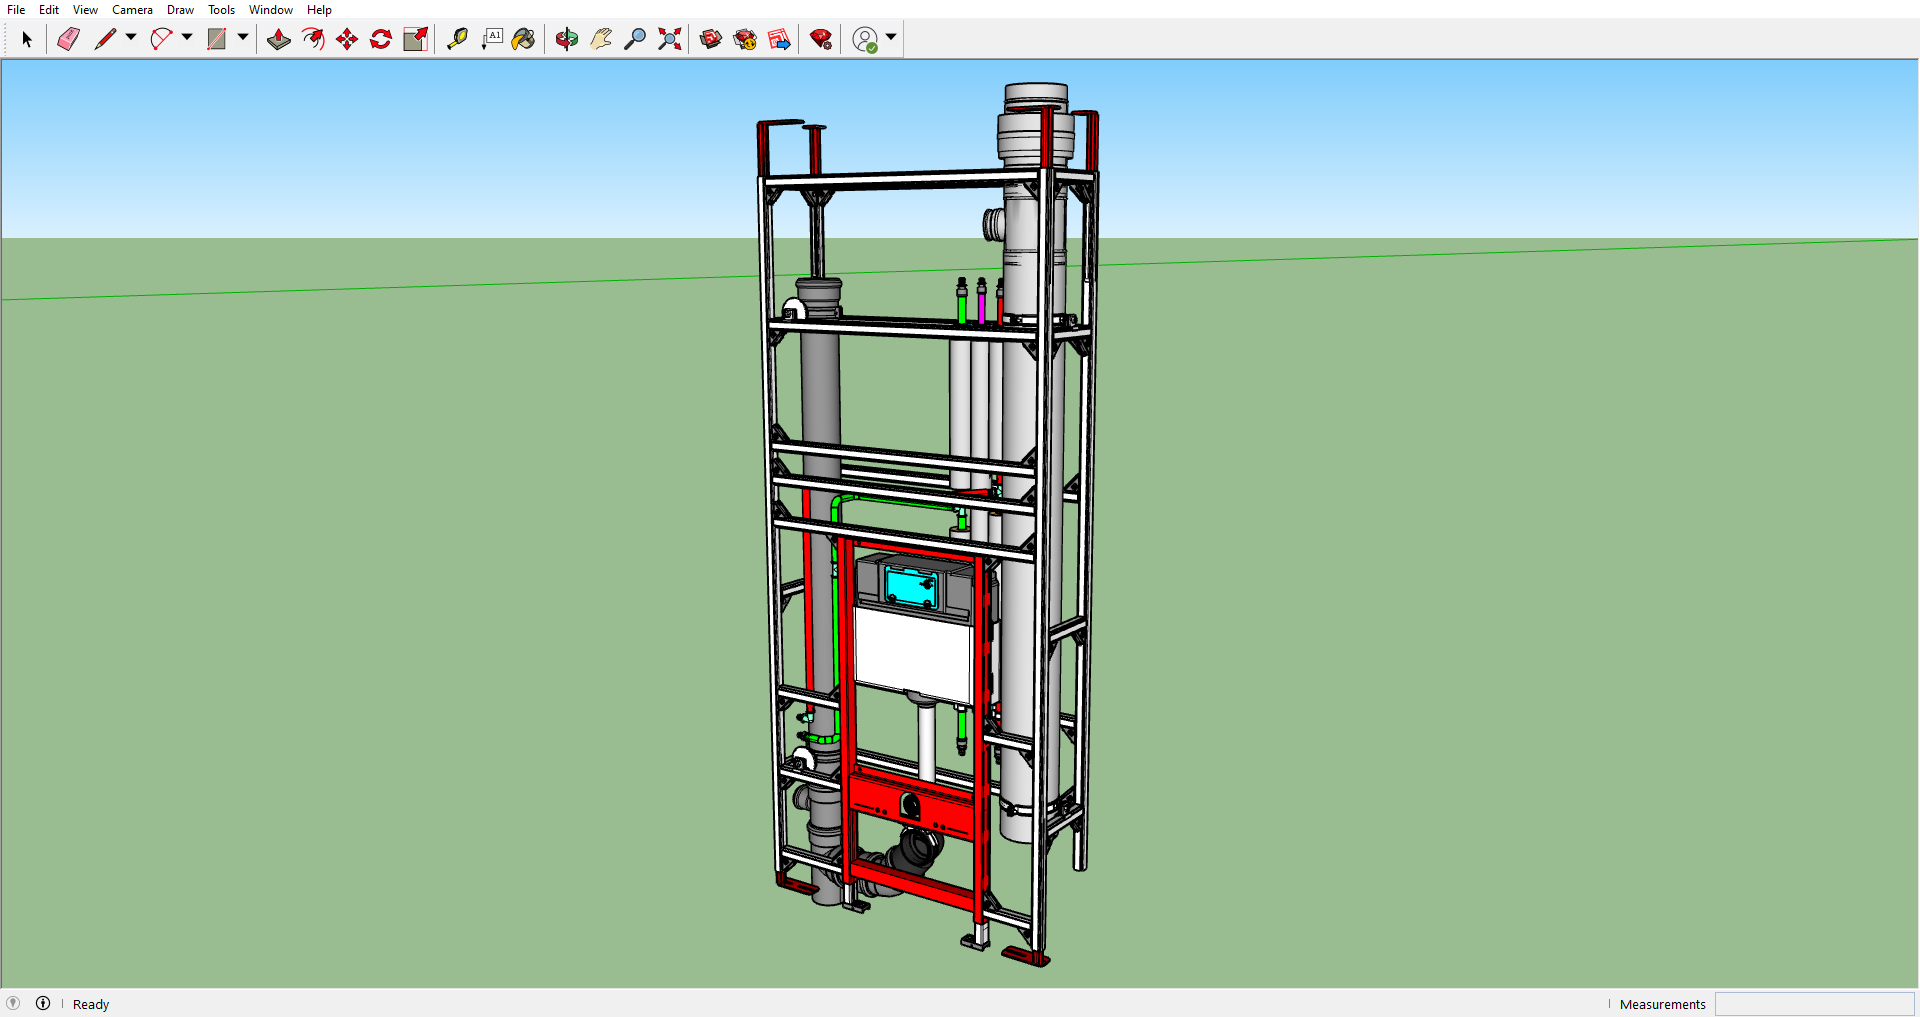
\includegraphics[width=1\textwidth]{images/sketchup.PNG}
    \caption{Das importiere WC - Register in SketchUp 2019}
    \label{fig:my_label}
\end{figure}
\\
Nach der Überprüfung wird das Modell in das Dateiformat .OBJ exportiert. \\ Außerdem werden die Material-Informationen in eine .MTL Datei exportiert. \\ \\
Im dritten Schritt wird das exportierte Paket, bestehend aus einer .OBJ, .MTL und beliebig vielen Bild - Dateien, in den blackthread.io/gltf-converter importiert. \\
\begin{figure}[h]
    \centering
    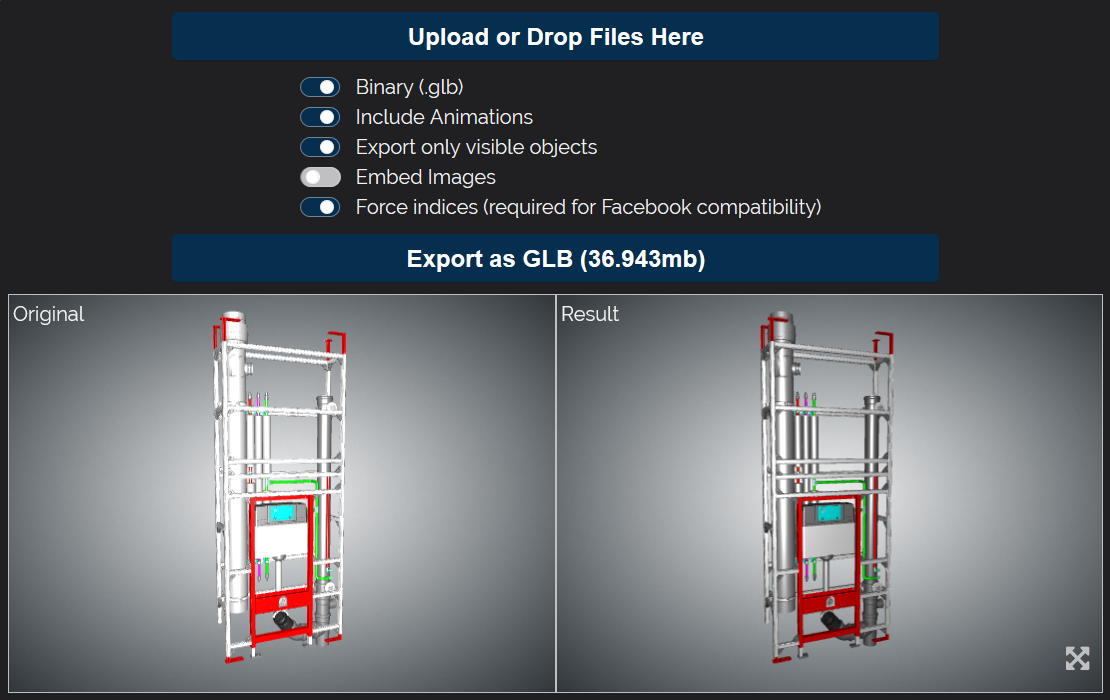
\includegraphics[width=1\textwidth]{images/converter.png}
    \caption{Das importierte WC - Register im GLTF/GLB - Converter \cite{Converter}}
    \label{fig:my_label}
\end{figure} 
\\
Im letzten Schritt wird das Modell als .GLB Datei exportiert.

\section{Modell laden}
Die exportierten .GLB - Modelle werden dann mit Three.js in das Tool geladen. \\
Um die bestmögliche Performance zu gewährleisten wird der GLTFLoader [\ref{sec:Loader}] benutzt. \\ Um Datenkompression einzubauen wird dem GLTFLoader ein DRACOLoader [\ref{dracoloader}] hinterlegt. Diese Konfiguration ermöglicht einen schnellen Ladevorgang.
\newpage
\subsection{JavaScript - Umsetzung}
Laden eines Modelles: 
\begin{lstlisting}
loadModel(object_name) {
    var loader = new THREE.GLTFLoader();
    
    var dracoLoader = new THREE.DRACOLoader();
    glbPath = 'models/' + object_name + '.glb';
    dracoLoader.setDecoderPath( 'js/libs/draco/' );
    dracoLoader.setDecoderConfig( { type: 'js' } );
    loader.setDRACOLoader( dracoLoader );
    //console.log(glbPath);
    // Load a glTF resource
    loader.load(
      // resource URL
      glbPath,
      // called when the resource is loaded
      function ( gltf ) {
        scene.add( gltf.scene );
        newObject = gltf.scene;
    
        onLoadComplete();
      },
      // called while loading is progressing
      function ( xhr ) {
      },
      // called when loading has errors
      function ( error ) {
        console.log( 'An error happened with ' + object_name);
      }
    );
}
\end{lstlisting}
Der DRACOLoader wird dem GLTFLoader mitgegeben, außerdem muss dem DRACOLoader ein Verweis auf eine JavaScript - Bibliothek übergeben werden. \\
In der \textit{load} Callback Funktion wird das Objekt der Szene hinzugefügt und danach wird eine Funktion aufgerufen die einige Konfigurationen am neu geladenen Objekt vornimmt. 
\newpage
\section{Modell - JSON - Struktur}\label{sec:Modell - JSON - Struktur}
Nach dem Ladevorgang der Modelle werden diese in ein Array abgespeichert. Standardmäßig im JSON-Format, diese Strukturierung der Daten macht es möglich die Modelle zu konfigurieren.
\begin{figure}[h]
    \centering
    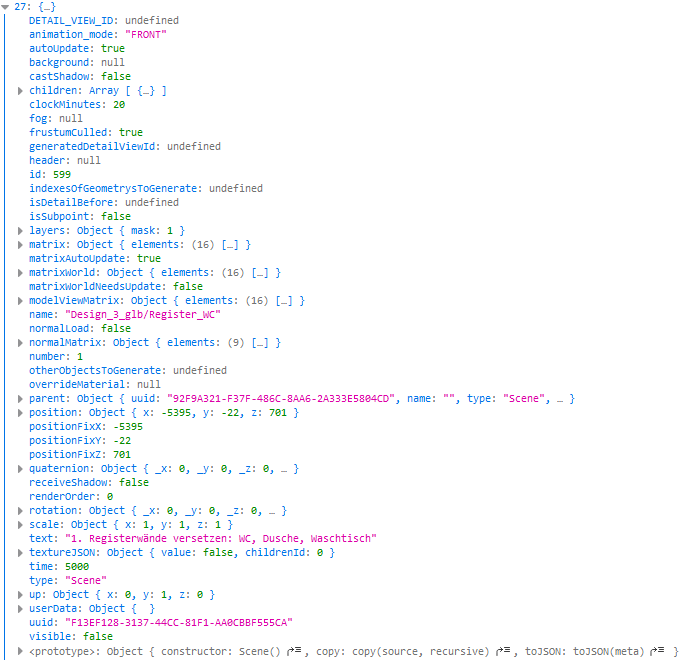
\includegraphics[width=0.8\textwidth]{images/json.PNG}
    \caption{JSON - Struktur des WC - Register Modells}
    \label{fig:my_label}
\end{figure} 
Informationen die mit dem Modell in Zusammenhang stehen, können durch die offene Struktur des JSON - Objekts einfach an dieses angehängt werden. \\
Beispiele für solch "angehängte Daten" wären:
\begin{itemize}
    \item .text \\
    Der Text der beim erscheinen des Modells in die Liste eingetragen werden soll.
    \item .textureJSON \\
    Ein JSON - Objekt das Informationen zur Textur und den jeweiligen Einstellungen dieser beinhaltet. 
    \item .clockMinutes \\
    Beinhaltet die \textit{virtuellen} Minuten die, die Uhr auf dem Bildschirm darstellen soll.
\end{itemize}
\newpage
\subsection{Modell - Position}
Die Position des ganzen Modells kann durch den Wert \textit{position} ausgelesen werden. \\
Um die Position einzelner Teile des Modells auszulesen muss dieser Wert ausgelesen werden:
\begin{lstlisting}
var element = object.children[0].children[x];
var x = element.geometry.boundingSphere.center.x
var y = element.geometry.boundingSphere.center.y
var z = element.geometry.boundingSphere.center.z
\end{lstlisting}
\subsection{Modell - Rotation}
Die Rotation des ganzen Modells kann man durch den Wert \textit{rotation} verändern. Hierbei muss beachtet werden, dass auf allen drei Verschiedenen Achsen rotiert werden kann.
\subsection{Modell - Skalierung}
Das Modell kann durch den Wert \textit{scale} skaliert werden, dies ist eine Alternative zum verändern der tatsächlichen Größe. Außerdem kann die Skalierung auf alle drei Achsen einzeln angewandt werden.
\subsection{Modell - Größe}
Die Maße der geladenen Modelle wird durch diesen Arbeitsdurchlauf nicht mitgespeichert und müssen so mit diesem Programmabschnitt neu berechnet werden:
\begin{lstlisting}
function setSize(object){
    var box = new THREE.Box3().setFromObject(object);
    const vector = new THREE.Vector3();
    box.getSize(vector);
    object.size = vector;
}
\end{lstlisting}
Grundsätzlich wird in diesem Code ein unsichtbarer Quader um das Modell dessen Größe berechnet werden soll erstellt. Die Größen dieses Quaders werden dann in einen Vektor abgespeichert und abschließend dem Objekt mit dem Parameter-Namen \textit{size} angehängt.
\newpage
\chapter{Animationen}

Animationen werden durch die JavaScript - Bibliothek \textit{Tween.js} [\ref{sec:tween.js}] realisiert. \\
Außerdem werden für den Animationsablauf, \textit{asynchrone Funktionen} genutzt.

\begin{lstlisting}
nextObject.position.y += 50;
var position = { y: nextObject.position.y};
var target = { y: nextObject.position.y - 50};
var tween = new TWEEN.Tween(position)
    .to(target, nextObject.time * MULTIPLIER);
tween.easing(TWEEN.Easing.Cubic.InOut);

tween.onUpdate(returnValue = function(){
    nextObject.position.y = position.y;
});
\end{lstlisting}
Die Variable \textit{nextObject} beinhaltet ein Modell im JSON - Format. [\ref{sec:Modell - JSON - Struktur}]
\\
In dieser Animation wird ein Objekt 50 Three.js - Längeneinheiten in die Höhe verschoben, um dann innerhalb des definierten Zeitraums wieder auf die Ausgangsposition zurückzukehren.
\begin{itemize}
    \item position: Ausgangsposition des Objekts.
    \item target: Zielposition des Objekts
    \item tween: Das TWEEN.js Objekt, Ausgangsposition, Zielposition und Animationszeitraum werden hinterlegt.
\end{itemize}
\textbf{Ablauf} \\
Das zu animierende Modell wird um einen festgelegten Wert nach oben verschoben. \\
Diese veränderte Position wird nun dem Ausgangsstandort, \textit{position} zugewiesen. \\
Dem Zielstandort, \textit{target} wird die Position des Objektes vor der Veränderung zugewiesen. \\
Nun wird ein neues TWEEN - Objekt erstellt, diesem wird die Ausgangsposition, \textit{position}, die Zielposition, \textit{target} und der vordefinierte Animationszeitraum, \textit{nextObject.time} übergeben. \\
Schließlich wird die \textit{onUpdate} Funktion des TWEEN - Objektes definiert. In dieser wird die tatsächliche Position des Modells auf die, zuvor inkrementierte Ausgangsposition gesetzt. \\
Die Animation ist beendet wenn die Zeit, \textit{nextObject.time} abgelaufen ist und damit zusammenhängend die Ausgangsposition ident zur Zielposition ist.
\newpage
\section{Kamera - Animationen}\label{sec:Kamera - Animationen}
In den Detailansichten des Bad-Designers wird die Kamerafahrt auch mit Tween.js [\ref{sec:tween.js}] realisiert.
Im folgendem Code werden die Kameraeinstellungen vorbereitet und abschließend die Animation definiert und gestartet.
\begin{lstlisting}
var currentDetailView = detailViews.find(dv => dv.id == detailViewId);
var from = {
    camera_x : camera.position.x,
    camera_y : camera.position.y,
    camera_z : camera.position.z,
    target_x : controls.target.x,
    target_y : controls.target.y,
    target_z : controls.target.z
};
var to = {
    camera_x : currentDetailView.camera.x,
    camera_y : currentDetailView.camera.y,
    camera_z : currentDetailView.camera.z,
    target_x : currentDetailView.target.x,
    target_y : currentDetailView.target.y,
    target_z : currentDetailView.target.z
};
var tween = new TWEEN.Tween(from)
    .to(to,2000 * MULTIPLIER)
    .easing(TWEEN.Easing.Linear.None)
    .onUpdate(function () {
        camera.position.set(from.camera_x, from.camera_y, from.camera_z);
        controls.target.x = from.target_x;
        controls.target.y = from.target_y;
        controls.target.z = from.target_z;
        controls.update();
    })
    .start();
\end{lstlisting}
\textbf{Ablauf} \\
Ausgangsposition und Blickwinkel der Kamera wird in \textit{from} abgespeichert. \\
Zielposition und Blickwinkel der Kamera wird in \textit{to} abgespeichert. \\
Dem TWEEN - Objekt werden die nötigen Daten übergeben. \\
In der \textit{onUpdate} - Funktion wird nun die Kameraposition und der Blickwinkel verändert.
\newpage
\chapter{Texturierung der Modelle}\label{sec:Texturierung der Modelle}
Über den Designmodus des Bad-Designers können Texturen auf die Modelle gelegt werden. Folgende Kapitel erläutern die Umsetzung.
\section{Verzeichnisstruktur}\label{sec:Verzeichnisstruktur}
Die Texturen werden am Server als .PNG Dateien bereitgestellt. \\
Wichtig ist hierbei die Benennung der Dateien. Diese müssen ident zu deren verbundenen Modelle benannt sein.
\begin{figure}[h]
    \begin{subfigure}{0.5\textwidth}
    \centering
    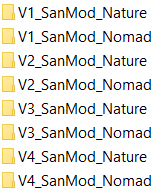
\includegraphics[width=0.7\linewidth]{images/ordner.PNG} 
    \caption{Verzeichnisstruktur pro Design}
    \label{fig:subim1}
    \end{subfigure}
    \begin{subfigure}{0.5\textwidth}
    \centering
    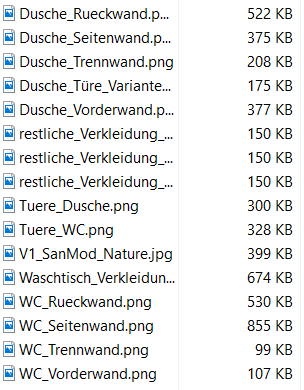
\includegraphics[width=0.6\linewidth]{images/texturenPngs.PNG}
    \caption{Texturen pro Modell}
    \label{fig:subim2}
    \end{subfigure}
\caption{Verzeichnisstruktur für die Texturierung der Modelle}
\label{fig:image2}
\end{figure}
\newpage
\section{Code: Konfiguration}\label{sec:Code: Konfiguration}
Die folgende Liste beinhaltet alle Daten die mit den Texturen zusammenhängen. 
\begin{itemize}
    \item id: Eine eindeutige Identifikationsnummer. 
    \item name: Der Verzeichnisname des zugehörigen Designs.
    \item displayName: Der Name des Designs der in der Auswahlliste für die jeweiligen Designs angezeigt wird.
    \item generatedTextureObjects: Eine Liste der generierten, texturierten Objekte.
    \item objectsToHide: Eine Liste der Objekte die zum Zeitpunkt der Designansicht unsichtbar gemacht werden sollten.
\end{itemize}
\begin{lstlisting}
textures.push(
{id: 1, name: 'V2_SanMod_Nature', displayName: 'NATURE', generatedTextureObjects: undefined, objectsToHide: undefined},
{id: 2, name: 'V2_SanMod_Nomad', displayName: 'NOMAD', generatedTextureObjects: undefined, objectsToHide: undefined});
\end{lstlisting}
Den Objekten wird folgendes JSON - Objekt schon kurz nach dem Ladeprozess hinterlegt.\\
Beispiel eines Texture-JSONs für \textit{restliche-Verkleidung-Dusche}:
\begin{lstlisting}
{value: true, childrenId: 0, hideAll: true, except: "V1_SanMod_Nature"}
\end{lstlisting}
\begin{itemize}
    \item value: Entweder true/false. Entscheidet ob für dieses Objekt Texturen verfügbar sind.
    \item childrenId: Legt fest welches Unter-Objekt des Modells für die Darstellung der Textur verwendet werden soll.
    \item hideAll: Entweder true/false. Entscheidet ob bei der Darstellung dieses texturierten Modells, alle Unter-Objekte unsichtbar gemacht werden sollen.
    \item except: Legt fest bei welchem Design für dieses Modell keine Textur hinterlegt ist.
\end{itemize}
\newpage
\section{Code: Generierung}
\begin{lstlisting}
function loadTextures(){
    textures.forEach(to => {
        var objectsWithTexture = objects.filter(o => o.textureJSON.value == true);
        var generatedTextureObjects = [];
        var objectsToHide = [];
        objectsWithTexture.forEach(o => {
            texturePath = 'models/texture/' + to.name + '/' + o.name.split('/')[1] + '.png';
            if(o.textureJSON.except == null || o.textureJSON.except != to.name){
                objectsToHide.push(o);
                png_texture = new THREE.TextureLoader().load(texturePath);
                png_material = new THREE.MeshPhongMaterial({ map: png_texture });
                png_material.transparent = true;
                png_material.side = THREE.DoubleSide;

                whiteMaterial = new THREE.MeshPhongMaterial();
                whiteMaterial.transparent = true;
                whiteMaterial.opacity = 0.50;

                materials = [png_material, png_material, whiteMaterial, png_material, png_material, undefined]

                mainMesh = o.children[0].children[o.textureJSON.childrenId];
                geometry = new THREE.BoxGeometry(mainMesh.size.x, mainMesh.size.y, mainMesh.size.z, 1, 1, 1, materials);
                generatedTextureObject = new THREE.Mesh(geometry, materials);
                mainMesh.geometry.computeBoundingSphere();

                //Position setzen...

                generatedTextureObjects.push(generatedTextureObject);
                scene.add(generatedTextureObject);
                generatedTextureObject.visible = false;
            }
        });
        to.generatedTextureObjects = generatedTextureObjects;
        to.objectsToHide = objectsToHide;
    });
}
\end{lstlisting}
Diese Funktion generiert für jedes Modell für das eine Textur verfügbar ist ein neues Modell mit der jeweiligen Textur. Dieser Lösungsweg wurde gewählt weil die nachträgliche Texturierung, geladener Modelle nicht möglich ist. \\
\textbf{Listen}
\begin{itemize}
    \item objectsWithTexture: Dieser Liste werden alle Objekte die texturiert werden müssen zugewiesen. Als Suchparameter wird der Wert \textit{value} des Texture - JSONs benutzt. [\ref{sec:Code: Konfiguration}]
    \item generatedTextureObjects: Dieser Liste werden im Laufe der Generierung alle generierten Objekte zugewiesen.
    \item objectsToHide: Dieser Liste werden im Laufe der Generierung alle originalen Objekte zugewiesen.
\end{itemize}
\textbf{Texturen und Materialien}
\begin{itemize}
    \item png\textunderscore texture: Die Textur die in dieser Iteration der Objekt-Liste geladen wurde.
    \item png\textunderscore material: Das Material dem die \textit{png\textunderscore texture} zugewiesen wird wurde.
    \item whiteMaterial: Ein Standard - \textit{MeshPhongMaterial} das für die Kanten des generierten Modells genutzt wird.
    \item materials: Ein Array der erstellten Materialien, für jede Seite des erstellen Objekts wird ein Material definiert. Die Rückseite des Modells benötigt keine Textur da, mit der Option \textit{material.side = THREE.DoubleSide} festgelegt wird das die Materialien von beiden Seiten sichtbar sind.
\end{itemize}
\textbf{Geometrien und Objekte}
\begin{itemize}
    \item mainMesh: Das Element des originalen Objekts, dass als Vorbild für das texturierte Objekt dient.
    \item geometry: Die Geometrie des generierten Objekts. Abmaße werden von \textit{mainMesh} übernommen und die Materialien werden hinterlegt.
    \item generatedTextureObject: Das fertig generierte Objekt, zusammengestellt aus der Geometrie und den Materialien.
\end{itemize}
\newpage
\section{Code: Texturen anzeigen}
Texturen werden durch die Auswahl eines Designs in der Designansicht angezeigt.\\
Folgender Code macht dies möglich:
\begin{lstlisting}
function showTexture(id){
    chosenTexture = textures.find(to => to.id == id);

    //Original-Objekte unsichtbar machen
    ANIMATING = true;
    chosenTexture.objectsToHide.forEach(o => {
        o.children[0].children[o.textureJSON.childrenId].visible = false;
        o.children[0].children.forEach(child => {
            if(child.type == "LineSegments"){
                child.visible = false;
            }
        });
        needsUpdate = true;
        
        //Parameter "hideAll" true?
        if(o.textureJSON.hideAll){
            o.children[0].children.forEach(c => {
                c.visible = false;
            });
        }
    });

    //Texturierte Objekte anzeigen
    chosenTexture.generatedTextureObjects.forEach(o => {
        o.visible = true;
    });
    ANIMATING = false;
}
\end{lstlisting}
In diesem Programmabschnitt werden die Texturen angezeigt. \\
\textbf{Ablauf:}
\begin{itemize}
    \item Das ausgewählte Textur - JSON - Objekt wird aus dem Array ausgelesen.
    \item Einzelne Elemente der Objekte ohne Textur werden unsichtbar gemacht.
    \item Es wird überprüft ob alle Elemente des Objekts unsichtbar gemacht werden sollen.
    \item Alle texturierten Objekte des ausgewählten Designs werden sichtbar gemacht.
\end{itemize}
Im ersten Abschnitt des Codes werden außerdem alle Elemente die vom Typ \textit{LineSegments} sind unsichtbar gemacht. \\
Diese Elemente sind hauptsächlich für das Zeichnen der Konturen zuständig und werden in diesem Teil der Darstellung nicht benötigt. \\
Im Bad-Designer spielen Elemente des Typs \textit{LineSegments} bei den Detailansichten eine große Rolle. Weil sie den Objekten auch bei sehr nahen Ansichten eine Struktur geben.
\newpage
\section{Code: Texturen unsichtbar machen}
Nach dem beenden des Designmodus wird die folgende Funktion aufgerufen:
\begin{lstlisting}
function endTextureMode(){
    //Texturierte Objekte unsichtbar machen
    if(chosenTexture != undefined){
        chosenTexture.generatedTextureObjects.forEach(o => {
            o.visible = false;
        });
        chosenTexture = undefined;
    }

    //Alle originalen Objekte/Modelle anzeigen
    objects.forEach(o => {
        o.children[0].children.forEach(child => child.visible = true);
    });
}
\end{lstlisting}
\textbf{Ablauf:}
\begin{itemize}
    \item Die generierten Objekte werden unsichtbar gemacht.
    \item Alle originalen Modelle werden sichtbar gemacht.
\end{itemize}
\section{Code: Neues Design hinzufügen}
Um ein neues Design zu implementieren, muss lediglich im \textit{textures} Array ein neues Element hinzugefügt werden und die Verzeichnisstruktur [\ref{sec:Verzeichnisstruktur}] eingehalten werden. \\ Hierbei ist zu beachten dass jedem Modell das im Texture - JSON - Objekt den Parameter \textit{value} den Wert \textit{true} zugewiesen hat, eine passende Textur im richtigen Format hinterlegt wurde. \\
Beispiel um ein neues Design hinzuzufügen:
\begin{lstlisting}
textures.push(
    {
        id: 3,
        name: 'V1_Test',
        displayName: 'TEST',
        generatedTextureObjects: undefined,
        objectsToHide: undefined
    }
);
\end{lstlisting}